
% a new beamer file for prague workshop

%% 
%%	This is file 'beamer_sample.tex'
%%	according to an MPIDR's PowerPoint template (?)
%%	
%%	by Eric Naujoks
%%
%%	Problems, bugs and comments to 
%%	naujoks@demogr.mpg.de
%%

%%%%%%%%%%%%%%%%%%%%%%%%%%%%%%%%%%
%%	Praelegomena								%%
%%%%%%%%%%%%%%%%%%%%%%%%%%%%%%%%%%
%%	- Make sure that you use utf8-encoding for all your .tex-files!!! (TeXnicCenter since version 2.0)
%%	- TeXnicCenter update: MPIDR intranet > Hard- & Sortfware > Software > Script and text editors > TeXnicCenter

\documentclass[20pt]{beamer}

\usepackage[ngerman,english]{babel}
\usepackage{graphicx}
\usepackage{tikz}
\usepackage{animate} 
\usepackage{amsmath}
\usepackage[normalem]{ulem}
\geometry{paperwidth=10in, paperheight=7.5in}
\usepackage{hyperref}
\usepackage[utf8]{inputenc}
\usepackage{multirow}
\usepackage{movie15}
%\usepackage{multimedia}
\usepackage{caption}
\captionsetup[figure]{labelformat=empty}
\usepackage[mpidr]{./mpidr/beamerthemeMPIDR}
\usepackage{array}
\newcolumntype{L}[1]{>{\raggedright\let\newline\\\arraybackslash\hspace{0pt}}m{#1}}
\newcolumntype{C}[1]{>{\centering\let\newline\\\arraybackslash\hspace{0pt}}m{#1}}
\newcolumntype{R}[1]{>{\raggedleft\let\newline\\\arraybackslash\hspace{0pt}}m{#1}}
\newcommand{\dd}{\; \mathrm{d}}
\newcommand{\tc}{\quad\quad\text{,}}
\newcommand{\tp}{\quad\quad\text{.}}

%% Declaring title and author
\title{Morbidity and Mortality}
\subtitle{Tim Riffe\\ Pil H. Chung\\ John MacInnes}
%% subtitle means author in this file...
% :/
%%	the institute's logo
\renewcommand{\mylogo}{
\includegraphics[width=5in]{logocustom}}


%%	should be the very last package to be loaded
\usepackage{hyperref}

%%%%%%%%%%%%%%%%%%%%%%%%%%%%%%%%%%
%%	Beginning of the document		%%
%%%%%%%%%%%%%%%%%%%%%%%%%%%%%%%%%%
\begin{document}
%%	titlepage - fixed frame:
%%	========================
\begin{frame}
	\titlepage
\end{frame}

%%	====
\begin{frame}%{Table of Contents}
\frametitle{The problem}
  \begin{description}
    \item<1->{\textbf{Projections}} show population \textbf{ageing}.
    \item<2->{\textbf{Robust}} mortality data, good projections.
    \item<3->{\textbf{Less reliable}} data on health. Less comparable.
    Cross-sectional surveys, subjective responses. Excluded populations.
    \item<4->{\textbf{Age-specific}} morbidity estimates key for predicting
    consequences of population ageing--- Social and health care demands.
  \end{description}
\end{frame}	



\begin{frame}
\frametitle{Some morbidity scenarios}
* assume mortality declines gradually, or similar.\\
* $Morb(a)$ is the chronological age pattern of morbidity
\begin{block}{Expansion}
\begin{description}
\item[1)] $Morb(a)$ $\uparrow$ (or
const) = morbidity vol. $\uparrow$
\item[2)] $Morb(a)$ $\downarrow$ but insufficient to offset mortality
                  decline = morbidity vol. $\uparrow$
\end{description}
\end{block}

\begin{block}{Compression}
\begin{description}
\item[3)]$Morb(a)$ $\downarrow$ fully offsets increased surv = constant morbidity
vol.
\item[4)] Fall in $Morb(a)$ outstrips mortality decline = morbidity vol. $\downarrow$
\end{description}
\end{block}

\end{frame}	

%%	section 1:
\begin{frame}%{Table of Contents}
\frametitle{Literature}

\begin{block}{Poor predictor}
Current $Morb(a)$ may be poor predictor of future $Morb(a)$
\end{block}

\begin{block}{Behaviours}
Impact of health behaviours: smoking, obesity, education, \ldots
\end{block}

\begin{block}{Innovation}
Tech innovation can change healthcare demand for given morbidity
\end{block}

\begin{block}{Pessimism}
General Pessimism, esp. using secenario 1 ($Morb(a)$ $\uparrow$, Surv $\uparrow$)
\end{block}
\end{frame}	%\end{frame}
%
\begin{frame}
\frametitle{more problems}
\begin{block}{Age standardization}
Chronological age standardization of conditions that are related with death can
degrade data rather than purge it of structure. Serious consequences.
\end{block}
\begin{block}{Assumptions}
\textbf{Chronological} age standardization makes morbidity follow OADR
\textbf{Thanatological} age standardization makes morbidity follow
the stock of population close to death.\footnotemark
\end{block}
%
\footnotetext{Remember Sanderson\& Scherbov (2005) ?}
\end{frame}

\begin{frame}

\begin{figure}[b]
\frametitle{~}
    \centering
    \caption{OADR vs REDR 1958-2009 various countries}
      % figure made in R/APClab.R
    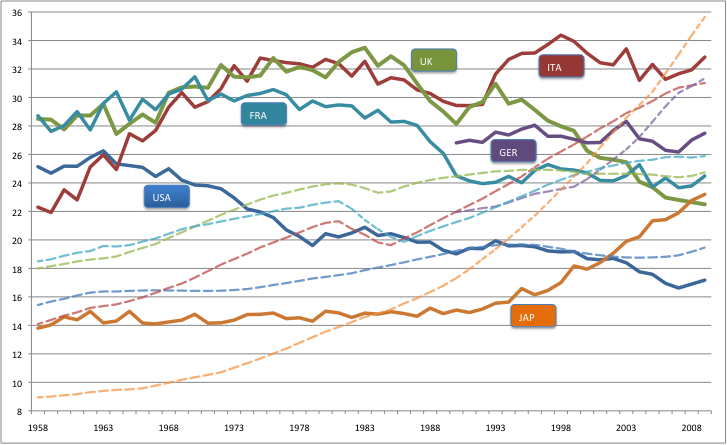
\includegraphics[scale=.9]{Figures/Johnsfig.png}
    %\caption{Lifelines in the APC diagram}
\end{figure} 
\end{frame}

\begin{frame}
\frametitle{Bigger problem}
\vspace{1em}
\begin{block}{~}
Chrono age standardisation typically leads to (very) pessimistic future
scenarios for volume of morbidity and assoc health/social care demand and
quality of life e.g., US CBO 250\% increase in GDP share going to elderly
support by 2050.
\end{block}
\vspace{-2em}
\begin{figure}[b]
    \centering
      % figure made in R/APClab.R
    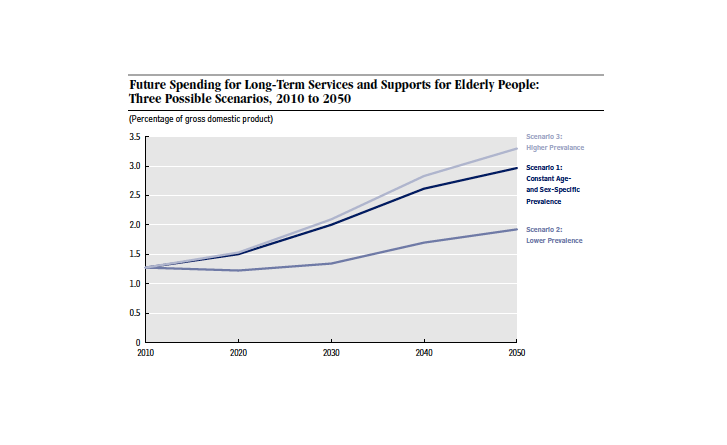
\includegraphics[scale=.9]{Figures/Johnsfig2.png}
    %\caption{Lifelines in the APC diagram}
\end{figure} 
\end{frame}

\begin{frame}
\frametitle{An alternative approach I}
\begin{block}{Understand temporal variation}
When broken down by both chronological and thanatological age, morbidity
conditions typically vary either as a function of thanatological age or as a
function of both age perspectives. Very few conditions are functions of
chronological age exclusively in elderly ages.
\end{block}

\end{frame}
\begin{frame}
\frametitle{An alternative approach II}
\begin{block}{Develop methods to deal with temporal variation}
Morbidity measurement is currently distorted by mortality. These
processes must be decoupled (for many conditions) in order to measure and
predict trends in morbidity and make sound predictions.
\end{block}
\end{frame}

\begin{frame}
\frametitle{A demonstration}
\begin{block}{Definitions}
\begin{description}
\item{$y$} is thanatological age 
\item{$a$} is chronological age 
\item{$J$} is a health condition that varies by $y$~~~\footnotemark
\item{$j(y)$} is the time-to-death function of $J$
\item{$j'(a)$} is the apparent chrono-age pattern of $J$
\item{$N(a)$} is population by age
\item{$\ell(a)$} is the survival function
\item{$\mu(a)$} is the force of mortality
\end{description}
\end{block}
\footnotetext{Imagine something that comes along with dying, even preceding it
by a decade, but doesn't kill you per say (This is includes many survey health questions\ldots)}
\end{frame}

\begin{frame}
\frametitle{A demonstration}
\begin{block}{Reasonable assumption?}
Is it reasonable to imagine $J$ as a function of only $y$? No, actually it's
more complicated than that, but for some conditions it appears to be pretty darn
close.
\end{block}
\end{frame}

\begin{frame}
\frametitle{A demonstration}
\begin{figure}[b]
    \centering
    \caption{ADL, 5 point index, HRS, USA Males, 1915 birth cohort\footnote{stuff life: eating, bathing, dressing, walking, getting
    up.}}
    \vspace{-3em}
      % figure made in R/APClab.R
    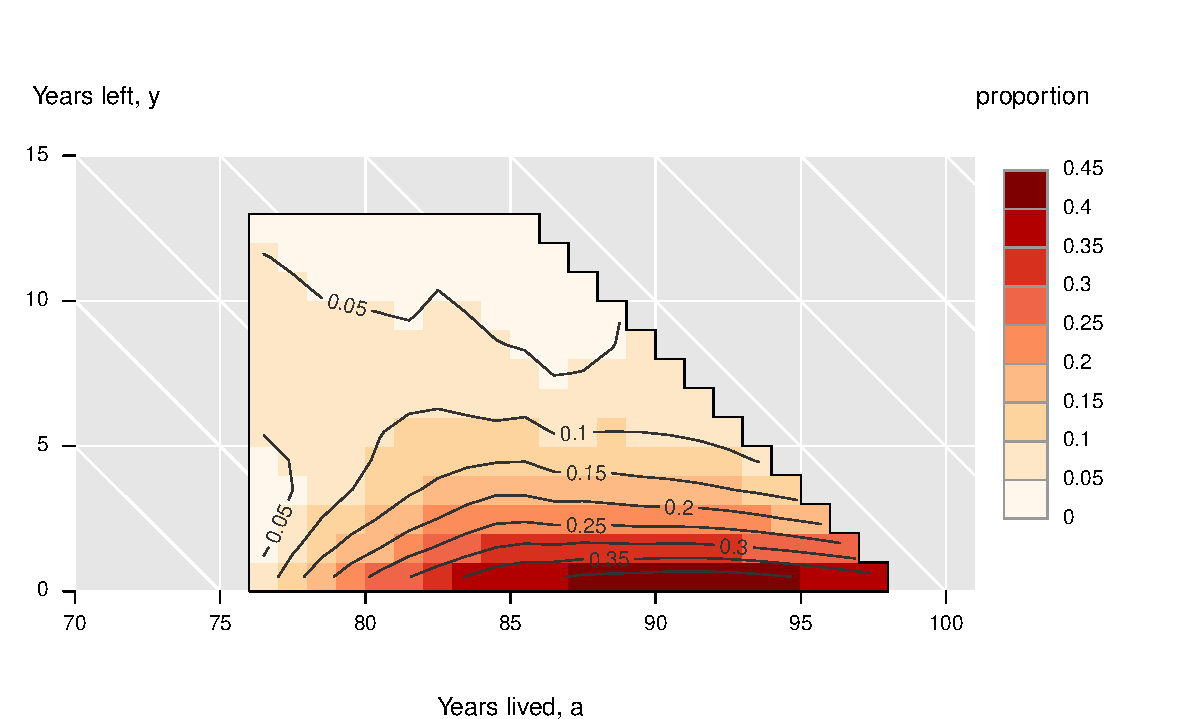
\includegraphics[scale=1.2]{Figures/SurfExample.pdf}
    %\caption{Lifelines in the APC diagram}
\end{figure} 
\end{frame}

\begin{frame}
\frametitle{A demonstration}
\begin{figure}[b]
    \centering
    \caption{ADL, 5 point index, HRS, USA Males, 1915 birth
    cohort}
    \vspace{-3em}
      % figure made in R/APClab.R
    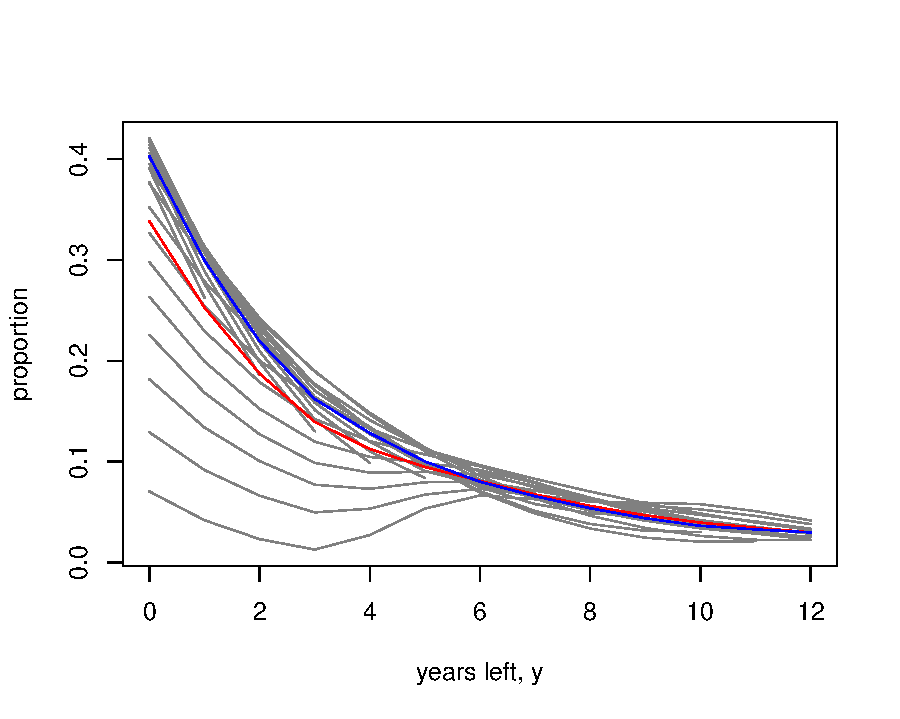
\includegraphics[scale=1.2]{Figures/LinesExample.pdf}
    %\caption{Lifelines in the APC diagram}
\end{figure} 
\end{frame}

\begin{frame}
\begin{block}{Reasonable assumption?}
Yes, it's not bad to assume something like $j(y)$ might exist, so we're free to
explore this assumption further. 
\end{block}

\begin{block}{red or blue line?}
It doesn't matter, we'd learn the same thing. Will use red here.
\end{block}
\end{frame}

\begin{frame}
\frametitle{For items like $j(y)$}

\begin{block}{$j(y)$ gives an age pattern}
Characteristics like $j(y)$ still have age patterns. They are tricky, shifty,
aggregates. The translation to chronological age depends on mortality.
\end{block}
\begin{align}
j'(a) &= \frac{\int _0^\omega j(y) N(a,y) \dd y}{N(a)} \\
      &= \frac{\int _0^\omega j(y) N(a) \mu(a+y)\frac{\ell(a+y)}{\ell(a)}\dd y}{N(a)}\\
      &= \int _0^\omega j(y) f(y|a)\dd y
\end{align}

\end{frame}

\begin{frame}
\frametitle{What does $j'(a)$ look like?}
\begin{figure}[b]
    \centering
    \caption{Period $j'(a)$, assuming the red $j(y)$. Familiar-looking
    curves?\footnotemark}
    \vspace{-3em}
      % figure made in R/APClab.R
    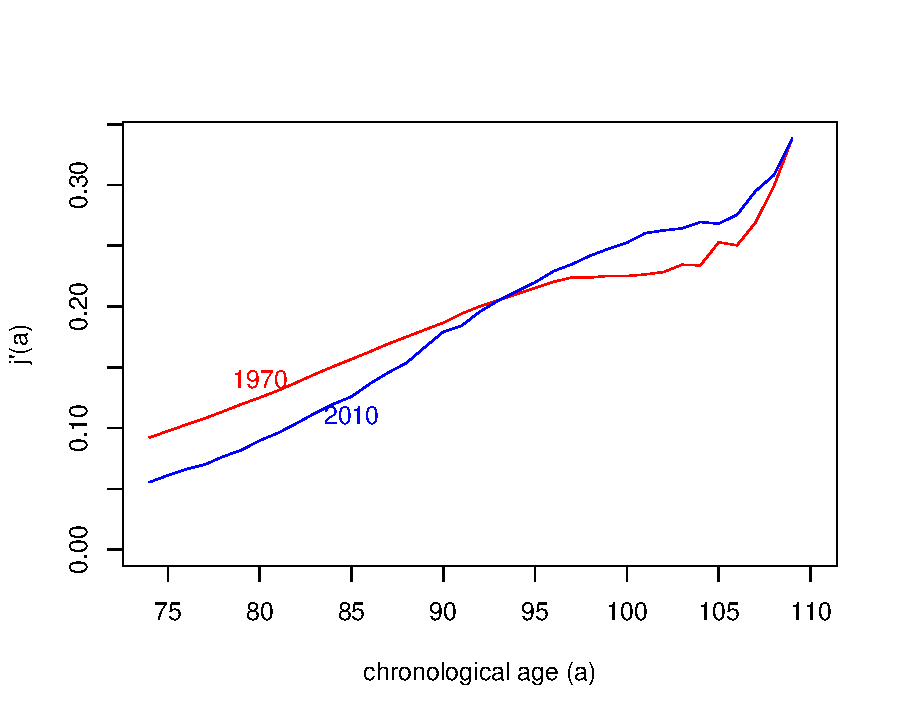
\includegraphics[scale=1.2]{Figures/jprimeaExample.pdf}
    %\caption{Lifelines in the APC diagram}
\end{figure} 
\footnotetext{Remember, we forced the same $j(y)$ on the whole series\ldots}
\end{frame}

\begin{frame}
\frametitle{What does $j'(a)$ predict?}
It's not so good at predicting\ldots
\begin{figure}[b]
    \centering
    \caption{2010 $J(a)$ predicted from 1970 $j'(a)$~~~~\footnotemark}
    \vspace{-3em}
      % figure made in R/APClab.R
    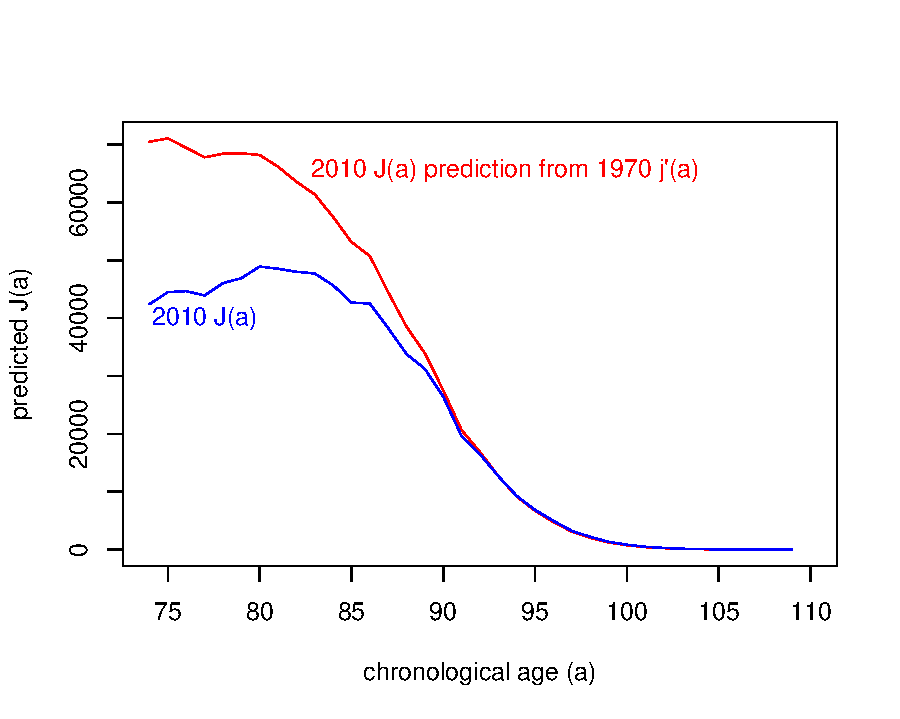
\includegraphics[scale=1.2]{Figures/jprimeaBadExample.pdf}
    %\caption{Lifelines in the APC diagram}
\end{figure} 
\footnotetext{This is a 30\% difference! The difference would have been bigger
given more mortality improvement.}
\end{frame}

\begin{frame}
\frametitle{An alternative}
\begin{block}{Measure more thoroughly}
Estimate $j(a,y)$ (surfaces), and predict the future with $j(a,y)$ together with
a mortality forecast. Needed: panel data with mortality followup, or registers
with good repeated health measures.
\end{block}
\end{frame}


\end{document}











